
%% Copyright 2019-2024 Elsevier Ltd
%% 
%% This file is part of the 'CAS Bundle'.
%% --------------------------------------
%% 
%% It may be distributed under the conditions of the LaTeX Project Public
%% License, either version 1.3c of this license or (at your option) any
%% later version.  The latest version of this license is in
%%    http://www.latex-project.org/lppl.txt
%% and version 1.3c or later is part of all distributions of LaTeX
%% version 1999/12/01 or later.
%% 
%% The list of all files belonging to the 'CAS Bundle' is
%% given in the file `manifest.txt'.
%% 
%% Template article for cas-sc documentclass for
%% single column output.

\documentclass[a4paper,fleqn]{cas-sc}

% If the frontmatter runs over more than one page
% use the longmktitle option.

%\documentclass[a4paper,fleqn,longmktitle]{cas-sc}

\usepackage[numbers]{natbib}
%\usepackage[authoryear]{natbib}
%\usepackage[authoryear,longnamesfirst]{natbib}
\usepackage{graphicx}
\usepackage{booktabs}
\usepackage{array}
\usepackage{algorithm}
\usepackage{algpseudocode}
\usepackage{enumitem}   
\usepackage{tabularx}

%%%Author macros
\def\tsc#1{\csdef{#1}{\textsc{\lowercase{#1}}\xspace}}
\tsc{WGM}
\tsc{QE}
%%%

\begin{document}
\let\WriteBookmarks\relax
\def\floatpagepagefraction{1}
\def\textpagefraction{.001}

% Short title
\shorttitle{TE-Q-Transformer for Battery SOH Estimation}

% Short author
\shortauthors{ZA Lisan et~al.}

% Main title of the paper
\title[mode=title]{TE-Q-Transformer: A Temperature-Embedded Quantum Framework for Battery State-of-Health Estimation}

% First author
\author[1]{Zadid Al Lisan}[orcid=0009-0001-1801-051X]
\ead{lisan15-5426@diu.edu.bd}

\author[1]{Md. Sulyman Islam Sifat}[orcid=0009-0005-6377-8973]

\ead{sifat15-4004@diu.edu.bd}

\author[3]{M.S. Hossain Lipu}[orcid=0000-0001-9060-4454] % replace XXXX with correct last 4 digits
\ead{molla_lipu@uow.edu.au}


\author[2]{Nazakat Ali}[orcid=0000-0002-3875-812X] % replace XXXX with correct last 4 digits
\ead{nazakat.ali@se.abb.com}



\author[1]{Md Alamgir Kabir}[orcid=0000-0002-7136-6339]
\ead{kabir.cse@diu.edu.bd}
\cormark[1]
%\credit{Conceptualization, Project administration, Writing – review \& editing, Supervision}

\affiliation[1]{organization={Department of Computer Science and Engineering, Daffodil International University},
            city={Dhaka},
            country={Bangladesh}}

\affiliation[2]{organization={ABB},
    city={Vasteras},
    country={Sweden}}

\affiliation[3]{organization={School of Electrical, Computer and Telecommunications Engineering, University of Wollongong},
    city={New South Wales 2522},
    country={Australia}}

    
% Corresponding author text
\cortext[1]{Corresponding author}
% Footnote text
\fntext[1]{}

\begin{abstract}
% Accurate state of health (SOH) estimation is fundamental to the safe and efficient operation of lithium-ion batteries in electric vehicles and renewable energy systems. Although battery degradation is influenced by various operating conditions, temperature remains one of the most critical factors affecting battery ageing. However, most data-driven SOH estimation models treat temperature as a standard input feature rather than explicitly modeling its impact on degradation. Consequently, their ability to generalize across unseen battery cells operating under different thermal conditions remains limited. To address this limitation, we propose a temperature-embedded quantum transformer named TE-Q-Transformer, a physics-informed hybrid quantum-classical framework that integrates Arrhenius-based ageing physics into quantum feature. The model embeds trainable activation-energy parameters within a 4-qubit quantum circuit to capture temperature-dependent degradation, followed by a lightweight transformer encoder for SOH estimation. The proposed framework is evaluated on two public benchmarks, the NASA battery dataset and the CALCE battery dataset, using a fixed hybrid cross-cell held-out split for each. On NASA, TE-Q-Transformer achieves an RMSE of 0.031, MAE of 0.026, and $R^2$ score of 0.516 against five representative baselines. On CALCE, the same architecture achieves an RMSE of 0.0409, MAE of 0.0334, and $R^2$ score of 0.870, again outperforming five baselines. These findings suggest that integrating Arrhenius-based ageing physics into quantum feature learning improves cross-cell generalization and enables more reliable SOH estimation across varying operating temperatures.
Accurate state of health (SOH) estimation is fundamental to the safe and efficient operation of lithium-ion batteries in electric vehicles and renewable energy systems. Although battery degradation is influenced by various operating conditions, temperature remains one of the most critical factors affecting battery ageing. However, most data-driven SOH estimation models treat temperature as a standard input feature rather than explicitly modeling its impact on degradation. Consequently, their ability to generalize across unseen battery cells operating under different thermal conditions remains limited. To address this limitation, we propose a temperature-embedded quantum transformer, TE-Q-Transformer, a physics-informed hybrid quantum-classical framework that integrates Arrhenius-based ageing physics into quantum feature. The model embeds trainable activation-energy parameters within a 4-qubit quantum circuit to capture temperature-dependent degradation. The proposed framework is evaluated on two public benchmarks, NASA and CALCE battery dataset. On NASA, TEQ-Transformer achieves an RMSE of 0.031, MAE of 0.026, and $R^2$ score of 0.516 against five representative baselines. On CALCE, the same architecture achieves an RMSE of 0.0409, MAE of 0.0334, and $R^2$ score of 0.870, outperforming five baselines. These findings suggest that integrating Arrhenius-based ageing physics into quantum feature learning improves cross-cell generalization and enables more reliable SOH estimation across varying operating temperatures.
\end{abstract}

% Research highlights
% \begin{highlights}
% \item We propose TE-Q-Transformer, a hybrid quantum-classical model for battery SOH estimation.
% \item An Arrhenius-informed quantum gate embeds thermal ageing physics directly into the model.
% \item The model gives the best cross-battery accuracy on the non-linear NASA dataset.
% % \item A fair NASA benchmark with a multi-temperature cross-cell held-out split is reported against five baseline models. The model is further validated on the CALCE dataset.
% \item The model is further validated on the CALCE dataset, where it again achieves the lowest RMSE and MAE and the highest $R^2$ among six models.
% \end{highlights}

% Keywords
\begin{keywords}
Quantum machine learning \sep Battery state of health \sep Hybrid quantum-classical model \sep Transformer \sep Arrhenius temperature encoding
\end{keywords}

\maketitle

% Main text
% Main text
\section{Introduction}\label{sec:intro}

Lithium-ion batteries play a central role in electric transport and energy storage because of their high energy density, long cycle life, and falling cost \citep{ralls2023role}. Reliable battery operation depends on the Battery Management System (BMS), which monitors the factors such as voltage, current, temperature, and State of Charge (SoC) to keep each cell within safe limits \citep{ali2025comprehensive}. Over time, battery State of Health (SOH), defined as the ratio of remaining usable capacity to the rated capacity, declines through mechanisms such as solid-electrolyte interphase (SEI) growth, lithium plating, and active material loss \citep{li2025deep}. Accurate SOH estimation is therefore needed for safe operation, longer battery life, and better energy management.

Among the factors that influence this degradation process, temperature is one of the most important. Low temperature slows lithium-ion transport and increases the risk of lithium plating, while high temperature accelerates SEI growth and electrolyte breakdown \citep{kumar2024,asiri2025}. Battery ageing is therefore strongly linked to thermal conditions. Most data-driven models (e.g., \citep{liu2025multi}, \citep{li2025unified}, \citep{yang2025physics} and \citep{sun2025battery}), however, treat temperature as a normal input feature rather than as a physical driver of degradation. As a result, they often fail to capture the non-linear thermal effects that shape SOH trajectories. This limitation becomes more serious when models must generalize beyond the conditions seen during training. Different cells can follow different ageing patterns because of differences in manufacturing, chemistry, and usage history \citep{lu2024mechanisms}. Cross-battery evaluation is therefore difficult, and random train-test splits can overstate model performance \citep{sedlavrik2025advanced}. Together, these issues highlight the need for an SOH estimation framework that combines thermal ageing physics with robust generalization across unseen batteries.

To address this gap, we propose Temperature-Embedded Quantum Transformer called TE-Q-Transformer, a hybrid model for SOH estimation from raw multi-channel battery sequences. First, temperature is mapped to a rotation angle through an Arrhenius-informed gate with trainable activation-energy linked to SEI growth and lithium plating. Besides, voltage, current, and normalized time are mapped to $\pi$-scaled rotations. Then, an expressive entangling circuit produces a quantum feature vector and is passed to a transformer encoder with CLS pooling and a small Multi-Layer Perceptron (MLP) head. The design keeps the overall pipeline lightweight relative to deep classical frameworks that is relevant for practical battery monitoring settings with limited compute resources.

% \citep{rahman2026}. 

The main contributions of this paper are as follows.
\begin{enumerate}[label=(\roman*)]
\item Model development: TE-Q-Transformer is proposed as a hybrid quantum-classical model in which an Arrhenius-informed temperature gate is incorporated, allowing thermal ageing effects to be embedded into the quantum state rather than treating temperature as a conventional feature. 
% for 
% for Li-ion battery SOH prediction by utilizing voltage, current, temperature, and time sequences.
% \item We introduce an Arrhenius-informed temperature gate that embeds thermal ageing effects into the quantum state instead of treating temperature as a normal feature.
\item Validation: A benchmark is presented on two public datasets, NASA and CALCE, using a hybrid cross-cell held-out protocol against classical and hybrid quantum-classical baselines.
\item Benchmarking and comparative analysis: The proposed framework demonstrates improvement on cross-battery generalization for Li-ion battery SOH prediction on both datasets. For reproduction of our proposed architecture, the codes are available online at \href{https://github.com/LisanHub/Te-Q-Transformer}{https://github.com/LisanHub/Te-Q-Transformer}.
% on the non-linear NASA dataset.
\end{enumerate}

The remainder of this paper is organized as follows. Section~\ref{sec:method} presents the methodology, including the NASA and CALCE datasets and preprocessing, the hybrid cross-cell held-out training protocols, the classical and hybrid quantum-classical baselines, and the proposed TE-Q-Transformer architecture with its Arrhenius-informed quantum embedding and Transformer stages. Section~\ref{sec:results} reports the experimental findings on the NASA benchmark, covering quantitative metrics against five baselines, cell-wise SOH trajectory analysis under the held-out thermal conditions, a component ablation of the proposed architecture, and an evidence-based analysis of the key claims, followed by a cross-dataset validation on CALCE. Section~\ref{sec:conclusion} concludes the paper and outlines directions for future work.

% \clearpage %%Remove this from your manuscript


\section{Related Work}\label{sec:related}

\subsection{Data-driven Battery SOH Estimation}\label{sec:rw-data}
Many studies have therefore turned to data-driven SOH methods on both laboratory and real-vehicle data. Such as Zhao et al. \citep{zhao2025capacity} fused a CNN-GRU model with Gaussian process regression and showed accurate capacity tracking on fleet data. Wang et al. \citep{wang2026lithium} validated their model on laboratory cells and a 260-vehicle real-world EV fleet. Moreover, Wen et al. \citep{wen2024lithium} used an interpretable boosting framework on pure electric vehicles and reported strong SOH accuracy under real charging behaviour. Furthermore, Liu et al. \citep{liu2025multi} proposed a multi-modal ResNet model on open-source field data and improved on common baselines such as SVR, random forest, GPR, and LSTM. Also, Sun et al. \citep{sun2025battery} applied a BO-XGBoost model with attention and also reached low estimation error. Together, these works show clear progress in learning from sequence data and large-scale vehicle records. However, most of them still feed temperature into the model in the same way as voltage and current. This limits their ability to represent Arrhenius-type thermal ageing \citep{gao2023effect}, which is one reason why performance can drop when models are tested on cells or operating conditions that differ from the training set. Since these classical models still struggle to represent the complex non-linear degradation mechanism, recent research has begun to explore hybrid quantum-classical learning as an alternative approach.

\subsection{Physics-guided and Temperature-aware SOH Estimation}\label{sec:rw-physics}
% TODO: No dedicated existing paragraph on physics-guided and temperature-aware SOH estimation was available to move without splitting or rewriting. Related sentences currently remain inside the Introduction motivation paragraph and the data-driven related-work paragraph.

\subsection{Quantum Machine Learning for Battery SOH Estimation}\label{sec:rw-qml}
Hybrid quantum-classical models have been studied for battery health prediction with the aim of learning non-linear degradation patterns under limited data. For example, Soon and Soon \citep{soon2025hybrid} combined a quantum neural network with a GRU and obtained high correlation with measured SOH on NASA cells. Similarly, Mutua et al. \citep{mutua2025} used a variational quantum neural network on NASA batteries and slightly outperformed a classical LSTM baseline. In another approach, Liang et al. \citep{liang2025stochastic} proposed a quantum convolutional neural network with automated feature fusion and reported clear RMSE gains over CNN, MLP, and LSTM models. Moreover, Wang et al. \citep{wang2024lithium} used a variational quantum algorithm with a stacking strategy and kept SOH error low on laboratory cells. More recently, Wang and Kebede \citep{wang2026prediction} applied a QLSTM with transfer learning on CAN-bus charging data from 20 vehicles and further improved prediction accuracy. These results suggest that quantum components can add useful non-linearity to SOH modelling. However, temperature is still rarely encoded as a physical mechanism inside the quantum circuit. In most quantum models, temperature is either treated like other sensor channels or handled through classical preprocessing before standard angle encoding. Therefore, there remains a need for a hybrid model that embeds temperature-driven ageing physics directly into quantum representations while preserving temporal sequence modelling capability.

\section{Methodology}\label{sec:method}

\begin{figure}
  \centering
    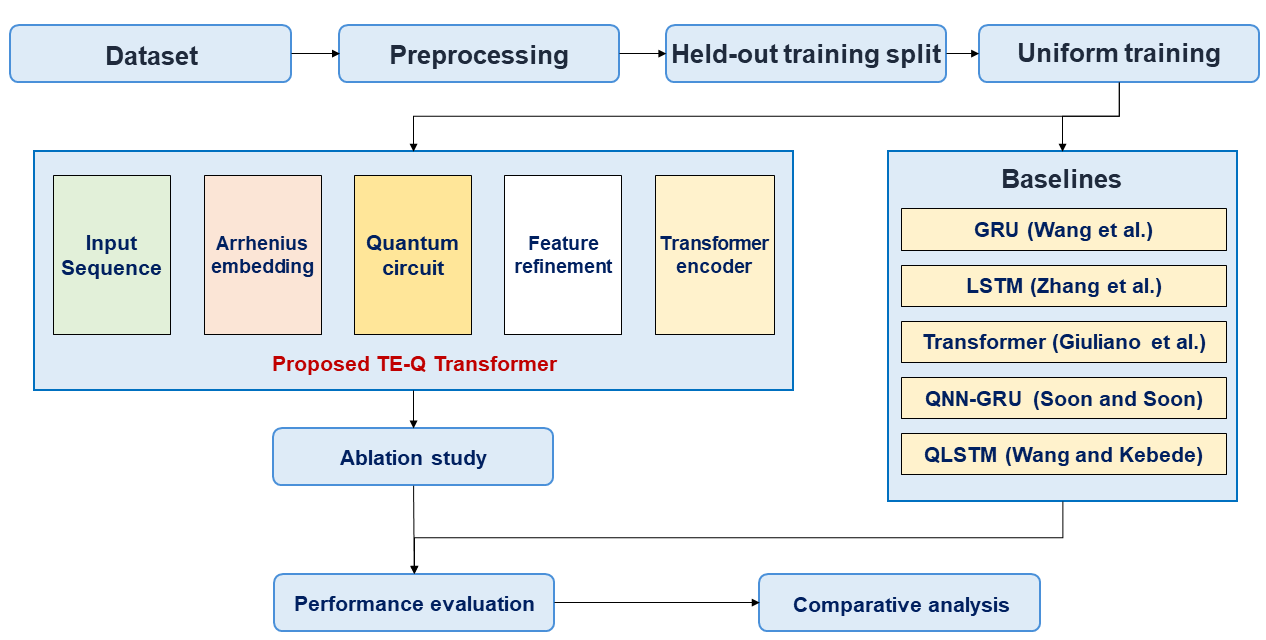
\includegraphics[width=\linewidth]{figs/teq_methodology.png}
    \caption{Overall workflow diagram }\label{methodology}
\end{figure}
This section describes the dataset, the training protocol, the baseline models, and the proposed TE-Q-Transformer framework. We pre-process the data and perform the experiment with a uniform training protocol across five baselines and our proposed model. We then conduct an ablation study before evaluating the performance along with comparative analysis. The overall workflow diagram is presented in Figure~\ref{methodology}. 

\subsection{Problem Formulation}\label{sec:problem}
% TODO: Problem formulation content to be added in manuscript revision.

\subsection{Datasets and Preprocessing}\label{sec:datasets}
To ensure that the proposed architecture is unbiased towards any specific dataset, we test TE-Q-Transformer on two publicly available datasets, NASA and CALCE.

The NASA battery dataset \cite{saha2007battery} is utilized as the primary benchmark since it has been adopted as a de facto standard for the evaluation of battery health estimation models \citep{komarsofla2026}. The dataset includes voltage, current and temperature readings at regular intervals during charge and discharge cycles. Since this study involves temperature embedding into quantum state, our NASA evaluation focuses on three thermally distinct cells: (i) B0018 at 24\,$^\circ$C, (ii) B0032 at 43\,$^\circ$C, and (iii) B0053 at 4\,$^\circ$C. This range from low to high ambient temperature supports our focus on temperature-aware SOH modelling.

As a second, independent benchmark, we use the CALCE battery dataset~\citep{w9rg-7173-25} from the Center for Advanced Life Cycle Engineering at the University of Maryland. Unlike NASA, the CALCE cells (CS2 series, lithium cobalt oxide prismatic cells) are cycled under a fixed ambient temperature and a constant-current constant-voltage protocol, so this dataset provides a cross-chemistry, cross-laboratory check on the generalization claims made on NASA rather than a further test of temperature-aware modelling. We use four CS2 cells for this benchmark: CS2\_35 and CS2\_36 form the full training set, CS2\_37 is split chronologically in the same way as B0053 on NASA, and CS2\_38 is reserved as a fully held-out test cell, with the same voltage, current, temperature, and normalized-time input channels as NASA.

For both datasets, SOH is defined per cell as the current measured capacity divided by that cell's first-cycle capacity. Each input window contains 512 time steps with four features: voltage, current, temperature, and normalized time. Only voltage, current, and normalized time are scaled with min-max normalization. The scaler is fitted on the training set only and then applied to the test set. Temperature is kept in raw degrees Celsius so that the Arrhenius gate receives physically meaningful values.

\subsection{Training and Evaluation Protocol}\label{sec:training}
We apply a fixed hybrid multi-temperature cross-cell held-out protocol inspired by recent studies (e.g. \citep{sahoo2022transfer}, \citep{che2023increasing}, and \citep{kumar2026temperature}).
Training and testing are strictly separated by cell identity, while data from one cell are divided based on time.
The full training set utilizes all recorded data from cells B0005, B0006, B0007, B0029, B0030, and B0031. Cells B0018 and B0032 are reserved as full test cells and never appear during training. Cell B0053 is split chronologically: the first 70\% of cycles are used for training and the remaining 30\% for testing (B0053\_test). Chronological order is preserved in all windows.

The same cross-cell held-out logic is applied to CALCE. Cells CS2\_35 and CS2\_36 contribute all of their cycles to training, cell CS2\_38 is reserved as a full test cell and never appears during training, and cell CS2\_37 is split chronologically with the first 70\% of cycles used for training and the remaining 30\% for testing (CS2\_37\_test). As on NASA, the min-max scaler used for voltage, current, and normalized time is fit on the CALCE training cells only, and chronological order is preserved within every window.

All models are evaluated with the same windowing, preprocessing, split rules, and metrics on both datasets. We report Root Mean Squared Error (RMSE), Mean Absolute Error (MAE), and the coefficient of determination (R\textsuperscript{2}). Table~\ref{tbl1} summarizes the training, windowing, and common architecture settings shared by all models on the NASA benchmark; the CALCE benchmark reuses the same windowing, scaling, optimization, and architecture settings, with the cell-level split described above.

\begin{table}%[]
\caption{Training, windowing, and common architecture settings for NASA dataset.}\label{tbl1}
\begin{tabular*}{\tblwidth}{@{}LL@{}}
\toprule
Item & Setting \\
\midrule
\multicolumn{2}{l}{\textit{Data and windowing}} \\
Input features & Voltage, Current, Temperature, Time (normalized) \\
Sequence length & 512 time steps per window \\
SOH definition & Current capacity divided by first-cycle capacity (per cell) \\
Preprocessing & Min-max scaling for voltage, current, and time (fit on train only). Temperature in raw $^\circ$C \\
Split protocol & Hybrid multi-temperature cross-cell held-out split \\
Training set & B0005--B0007, B0029--B0031, first $70\%$ of B0053 \\
Test set & B0018, B0032, remaining $30\%$ of B0053 \\
Evaluation metrics & RMSE, MAE, R\textsuperscript{2} \\
\midrule
\multicolumn{2}{l}{\textit{Common architecture}} \\
Model dimension & $d_{\mathrm{model}}=64$ \\
Encoder depth & 1 layer \\
Dropout & 0 \\
Regression head & $\mathrm{Linear}(64,64)$ $\rightarrow$ GELU $\rightarrow$ $\mathrm{Dropout}$ $\rightarrow$ $\mathrm{Linear}(64,1)$ \\
\midrule
\multicolumn{2}{l}{\textit{Optimization and training}} \\
Optimizer & AdamW; learning rate $10^{-3}$; weight decay $5\times10^{-2}$ \\
Loss function & Mean squared error (MSE) \\
Learning-rate scheduler & ReduceLROnPlateau; factor $0.5$; patience $10$ \\
Gradient clipping & Maximum norm $1.0$ \\
Early stopping & Patience $20$ based on training loss \\
Training epochs & $80$ \\
Batch size & $8$ \\
\bottomrule
\end{tabular*}
\end{table}

\subsection{Baseline Models}\label{sec:baselines}
We compare TE-Q-Transformer with five baselines from recent SOH estimation studies (i.e., \citep{wang2024state, zhang2023accurate, giuliano2025transformer, soon2025hybrid, wang2026prediction}). There are two types of baselines: deep learning sequence models and hybrid quantum-classical models. 

Three classical architectures that learn SOH directly from temporal sensor data comprise the deep learning group. The following are examples of these:  
\begin{enumerate}[label=(\roman*)]
  \item \textbf{Wang et al.~\citep{wang2024state}:} This study combined empirical mode decomposition with Random Forest and GRU networks for battery health estimation.  They used charge and discharge voltage curves to extract time-based features, decomposed capacity data into smoother components, and used various models to the fluctuating and steady parts. This design enhanced the accuracy of the data and decreased the computation time for NASA battery information. We take this approach as the GRU baseline.
  \item \textbf{Zhang et al.~\citep{zhang2023accurate}:} The authors utilized a LSTM network that that monitors the battery capacity degradation with time. The capacity was used as the primary health indicator and history was fed into the model in the form of sequences of ages. Tests on NASA batteries showed that the approach can predict remaining capacity and remaining useful life reliably. We consider this method as our LSTM baseline.
  \item \textbf{Giuliano et al.~\citep{giuliano2025transformer}:} They proposed a Transformer that uses attention to capture long-term ageing trends across battery cycles. They studied transfer from one battery type on the NASA dataset to another chemistry on the Oxford dataset. After fine-tuning, the Transformer improved accuracy and outperformed models trained only on the target data. This architecture is used as our Transformer baseline.
\end{enumerate}

Furthermore, the hybrid quantum-classical group combines quantum circuits with classical sequence learning. These are given below:
\begin{enumerate}[label=(\roman*)]
  \item \textbf{Soon and Soon \citep{soon2025hybrid}:} The authors paired a quantum neural network with a classical GRU forming QNN-GRU. They used three easy-to-measure discharge features as inputs. The hybrid model achieved lower prediction error than several standard machine learning methods on NASA batteries. This design corresponds to our QNN-GRU baseline.
  \item \textbf{Wang and Kebede \citep{wang2026prediction}:} They developed a quantum-enhanced LSTM (QLSTM) with shared embedding layers and transfer learning for electric-vehicle battery pack health estimation. 
  % The method was designed for partial real-world charging data collected from multiple vehicles over many months. 
  % Training on several packs together gave better accuracy than training on a single pack, with very low prediction error. 
  This approach is implemented as our QLSTM baseline.
\end{enumerate}

Table~\ref{tab:nasa_baseline_config} reports the model-specific configurations of these five baselines, including feature projection, sequence encoder, attention, feed-forward width, quantum circuit, positional encoding, and sequence representation. The same five configurations, without any dataset-specific tuning, are reused for the CALCE benchmark in Section~\ref{sec:calce}, so that differences in accuracy between the two datasets reflect the data itself rather than a change in baseline design.

\begin{table*}[t]
\centering
\caption{Model-specific configurations of the baseline models evaluated on the NASA battery dataset. Shared architecture, optimization, and data-processing settings are listed in Table~\ref{tbl1}.}
\label{tab:nasa_baseline_config}
\footnotesize
\setlength{\tabcolsep}{4pt}
\renewcommand{\arraystretch}{1.18}

\begin{tabular}{>{\raggedright\arraybackslash}p{0.16\textwidth}
                >{\centering\arraybackslash}p{0.16\textwidth}
                >{\centering\arraybackslash}p{0.16\textwidth}
                >{\centering\arraybackslash}p{0.16\textwidth}
                >{\centering\arraybackslash}p{0.16\textwidth}
                >{\centering\arraybackslash}p{0.16\textwidth}}
\toprule
\textbf{Configuration} &
Wang et al.~\newline\citep{wang2024state} &
Zhang et al.~\newline\citep{zhang2023accurate} &
Giuliano et al.~\newline\citep{giuliano2025transformer} &
Soon and Soon\newline\citep{soon2025hybrid} &
Wang and Kebede\newline\citep{wang2026prediction} \\
\midrule

Feature projection
& $\mathrm{Linear}(4,64)$
& $\mathrm{Linear}(4,64)$
& $\mathrm{Linear}(4,64)$
& $\mathrm{Linear}(4,4)$ $\rightarrow$ QNN $\rightarrow$ $\mathrm{Linear}(4,64)$
& $\mathrm{Linear}(4,4)$ $\rightarrow$ QNN $\rightarrow$ $\mathrm{Linear}(4,64)$ \\

Sequence encoder
& GRU
& LSTM
& Transformer Encoder
& GRU
& LSTM \\

Attention mechanism
& None
& None
& 4 attention heads
& None
& None \\

Feed-forward dimension
& --
& --
& $256$
& --
& -- \\

Quantum circuit
& --
& --
& --
& 4 qubits, 2 layers$^{\mathrm{a}}$
& 4 qubits, 2 layers$^{\mathrm{a}}$ \\

Positional encoding
& --
& --
& Sinusoidal
& --
& -- \\

Sequence representation
& Last hidden state
& Last hidden state
& Last token
& Last hidden state
& Last hidden state \\

\bottomrule
\end{tabular}

\vspace{3pt}
\begin{minipage}{0.98\textwidth}
\footnotesize
\textit{Note:}
$^{\mathrm{a}}$ The quantum circuit uses Y-axis AngleEmbedding, 
BasicEntanglerLayers, and Pauli-$Z$ expectation measurements implemented
with PennyLane \texttt{default.qubit} on CPU. The sinusoidal positional
encoding uses a maximum sequence length of $512$.
\end{minipage}

\end{table*}



\subsection{Proposed TE-Q-Transformer Architecture}\label{sec:architecture}
The proposed model, TE-Q-Transformer, predicts battery state of health from sensor data using a five-stage pipeline. The model embeds known battery degradation physics directly into its input representation using a quantum circuit, then processes the resulting features over time with a transformer encoder to capture long-range temporal patt+erns. Figure~\ref{fig1} shows the full pipeline of the proposed model with five phases.

\begin{figure}
  \centering
    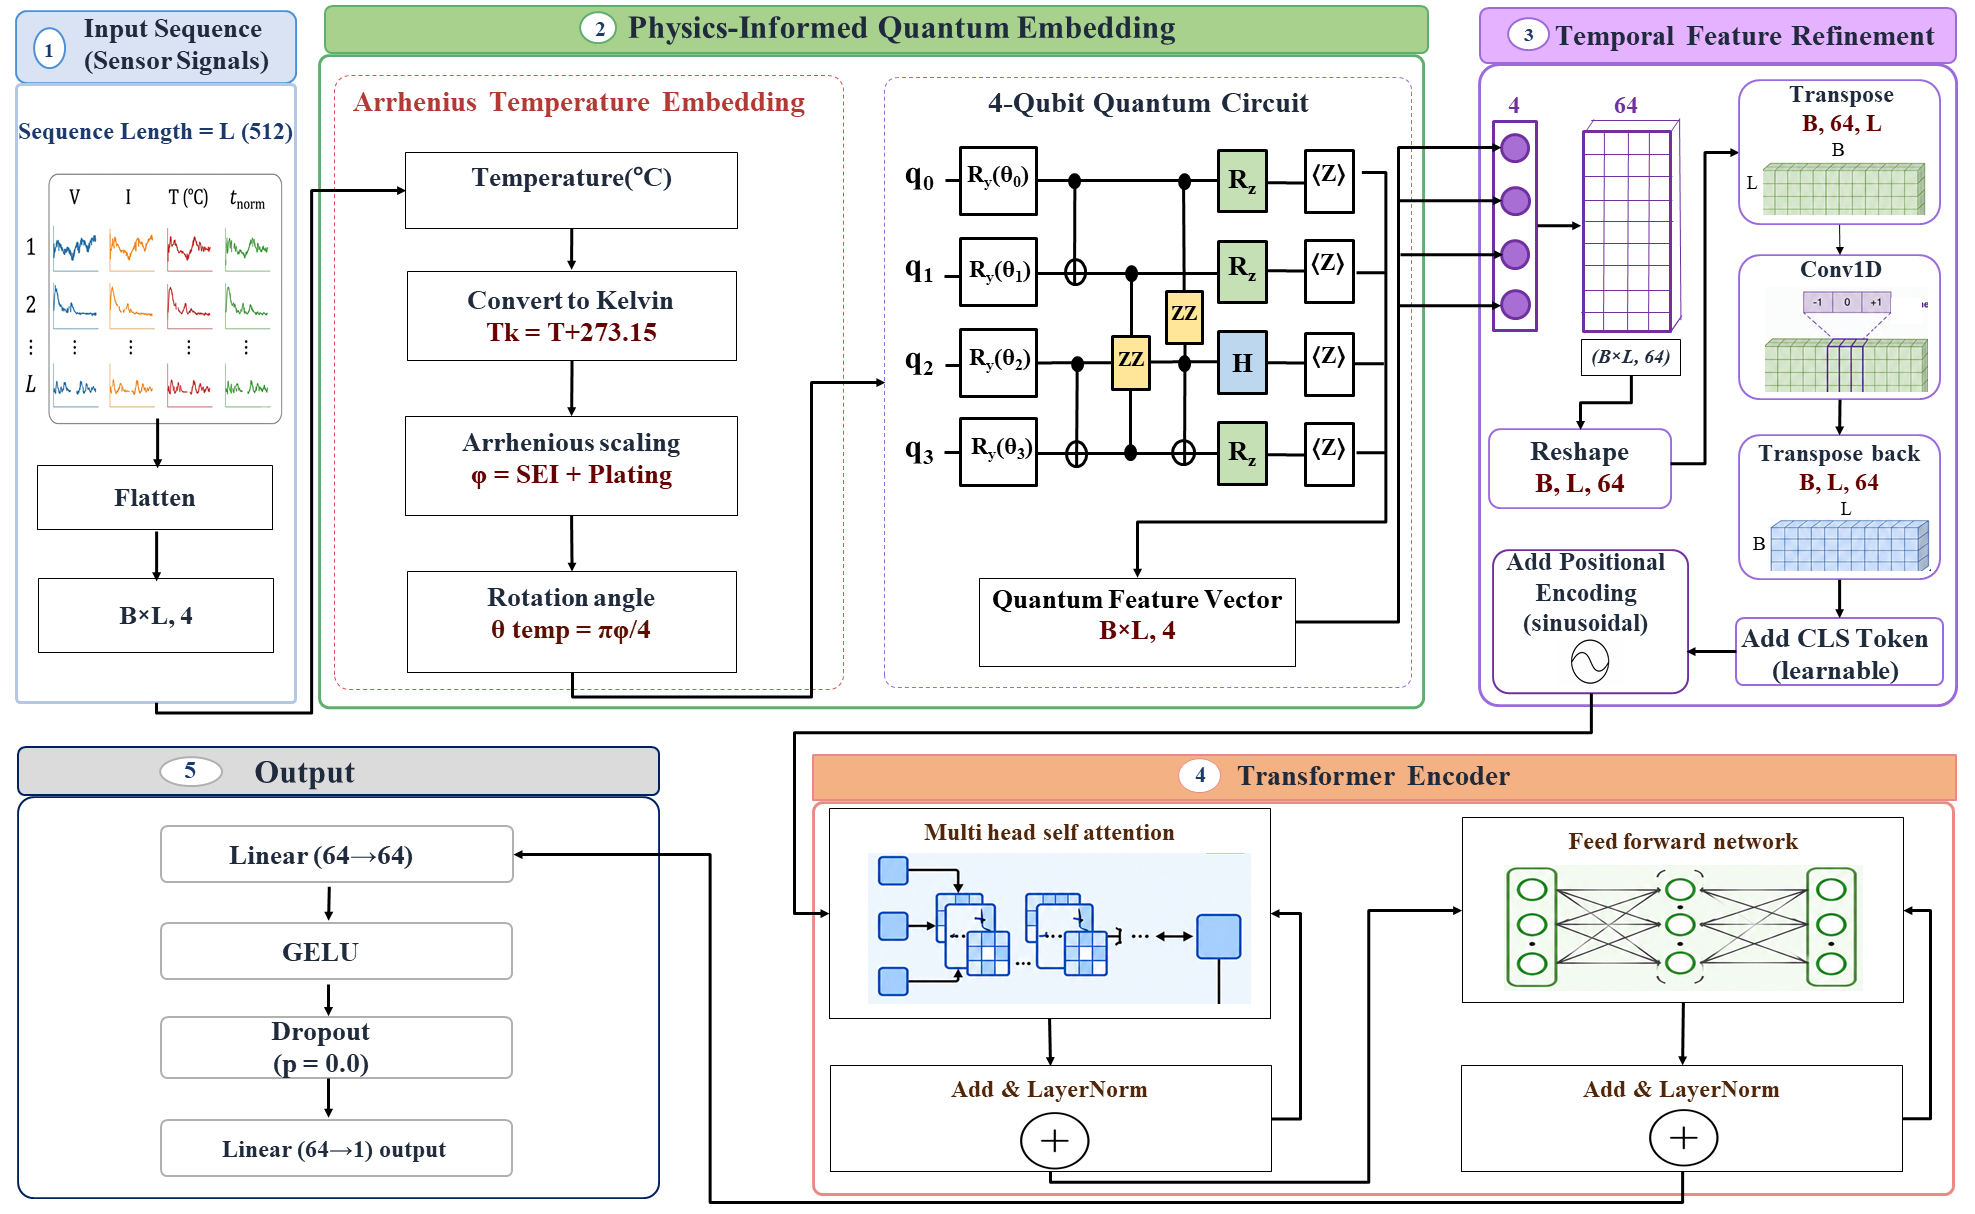
\includegraphics[width=\linewidth]{figs/teq_architecture.png}
    \caption{TE-Q-Transformer architecture: (1) input sensor sequence, (2) physics-informed quantum embedding with Arrhenius temperature gate, (3) temporal feature refinement, (4) Transformer encoder, and (5) SOH output head.}\label{fig1}
\end{figure}

\subsubsection{Phase 1: Input Sensor Sequence} The model receives a batch of input windows with shape $(B, L, 4)$, where $B$ is the batch size, $L=512$ is the sequence length, and the four features are voltage $V$, current $I$, temperature $T$ in degrees Celsius, and normalized time $t_{\mathrm{norm}}$. Temperature is kept in raw degrees Celsius so that the Arrhenius gate can use physical thermal values. The other three features are min-max scaled with a scaler fitted on the training set only to avoid data leakage. Finally, the tensor is then flattened to $(B \cdot L, 4)$ shape so that each time step can be processed independently by the quantum layer.

\subsubsection{Phase 2: Physics-informed Quantum Embedding with Arrhenius Temperature Gate}
The second phase converts each time-step reading into a small quantum feature vector. Instead of feeding temperature into the circuit as an ordinary scaled input, the model first uses well-known battery ageing physics to decide how strongly temperature should influence the quantum state. That idea is implemented in two consecutive layers: an Arrhenius temperature layer and a four-qubit quantum circuit. The Arrhenius layer focuses on two temperature-sensitive ageing processes that matter for lithium-ion cells. Solid electrolyte interphase (SEI) growth is one common source of capacity fade, and lithium plating becomes more relevant under cold operating conditions. The network learns two activation-energy parameters, $E_{a,\mathrm{sei}}$ and $E_{a,\mathrm{pl}}$, so that the embedding can adapt to how strongly each process should respond to temperature during training. Before those factors are computed, the measured temperature $T$ in degrees Celsius is converted to an absolute temperature $T_K$ in Kelvin by Eq.~\eqref{eq:kelvin}. It keeps the thermal input in physical units and avoids non-physical Kelvin values at the lower end.
\begin{equation}
T_K = \max(T + 273.15,\, 1). \quad \cite{waldmann2014temperature}
\label{eq:kelvin}
\end{equation}
A reference temperature $T_{\mathrm{ref}} = 298.15$\,K and the gas constant $R = 8.314$\,J\,mol$^{-1}$\,K$^{-1}$ are used in the Arrhenius terms below. The SEI-related thermal factor $\phi_{\mathrm{sei}}$ is demonstrated in Eq.~\eqref{eq:arrhenius-sei}. It increases or decreases the SEI contribution relative to room temperature, using $T_K$ from Eq.~\eqref{eq:kelvin}. 
\begin{equation}
\phi_{\mathrm{sei}} = \exp\!\left(\frac{E_{a,\mathrm{sei}} \cdot 10^{4}}{R}\left(\frac{1}{T_{\mathrm{ref}}} - \frac{1}{T_K}\right)\right). \quad \cite{kucinskis2022arrhenius}
\label{eq:arrhenius-sei}
\end{equation}
A separate Arrhenius term $\phi_{\mathrm{pl}}$ models lithium plating with the exponent arranged so that cold-temperature behaviour can be learned independently of SEI by Eq.~\eqref{eq:arrhenius-pl}.
\begin{equation}
\phi_{\mathrm{pl}} = \exp\!\left(\frac{E_{a,\mathrm{pl}} \cdot 10^{4}}{R}\left(\frac{1}{T_K} - \frac{1}{T_{\mathrm{ref}}}\right)\right). \quad \cite{yang2018understanding}
\label{eq:arrhenius-pl}
\end{equation}
Eq.~\eqref{eq:arrhenius-sei} works together with Eq.~\eqref{eq:arrhenius-pl} to form a combined thermal signal. That signal is turned into the temperature rotation angle $\theta_T$ by Eq.~\eqref{eq:theta-temp}.
\begin{equation}
\theta_T = \frac{\pi}{4}\left(\phi_{\mathrm{sei}} + \phi_{\mathrm{pl}}\right). \quad \cite{gao2017efficient}
\label{eq:theta-temp}
\end{equation}
Eq.~\eqref{eq:theta-temp} therefore links measured temperature to the quantum embedding through degradation physics rather than a fixed scaling rule. 


The four-qubit circuit is the second part of this stage. Voltage, current, and normalized time are already scaled to $[0,1]$; each channel is mapped to its own rotation angle on one qubit, while $\theta_T$ from Eq.~\eqref{eq:theta-temp} drives the temperature qubit. The voltage rotation angle $\theta_V$ is defined in Eq.~\eqref{eq:theta-v}.
\begin{equation}
\theta_V = \pi V. \quad \cite{hirai2024practical}
\label{eq:theta-v}
\end{equation}
Eq.~\eqref{eq:theta-v} maps the normalized voltage to a rotation in $[0,\pi]$. The current and time channels use the same linear mapping to angles $\theta_I$ and $\theta_t$ in Eq.~\eqref{eq:theta-i-t}.
\begin{equation}
\theta_I = \pi I, \qquad \theta_t = \pi t_{\mathrm{norm}}. \quad \cite{ovalle2023quantum}
\label{eq:theta-i-t}
\end{equation}
Eq.~\eqref{eq:theta-i-t} supplies the remaining input angles together with Eq.~\eqref{eq:theta-v} and Eq.~\eqref{eq:theta-temp}. Each angle is applied as an $R_y$ rotation on qubits $q_0$--$q_3$, which together form the encoding unitary $U_{\mathrm{enc}}$. The qubits are then mixed through a rich entangling unitary $U_{\mathrm{rich}}$ ($R_z$ gates, CNOTs, neighbouring Ising $ZZ$ couplings, Toffoli gates, Hadamard gates, and a closing $R_z$). Starting from the four-qubit ground state $\lvert 0\rangle^{\otimes 4}$, the resulting quantum state $\lvert\psi\rangle$ is given by Eq.~\eqref{eq:psi}.
\begin{equation}
\lvert\psi\rangle
=
U_{\mathrm{rich}}\,
U_{\mathrm{enc}}(\theta_V,\theta_I,\theta_t,\theta_T)\,
\lvert 0\rangle^{\otimes 4}.
\label{eq:psi}
\end{equation}
Eq.~\eqref{eq:psi} applies the angle embedding and the rich entangler to the four-qubit ground state. The circuit is simulated in PennyLane and trained end to end with backpropagation. Measuring the Pauli-$Z$ operators $Z_{0}$, $Z_{1}$, $Z_{2}$, and $Z_{3}$ on the four qubits yields the feature vector $\mathbf{q}$ in Eq.~\eqref{eq:pauli-z}.
\begin{equation}
\mathbf{q}
=
\bigl[
\langle\psi\rvert Z_{0}\lvert\psi\rangle,\,
\langle\psi\rvert Z_{1}\lvert\psi\rangle,\,
\langle\psi\rvert Z_{2}\lvert\psi\rangle,\,
\langle\psi\rvert Z_{3}\lvert\psi\rangle
\bigr]^{\top}.
\label{eq:pauli-z}
\end{equation}
Eq.~\eqref{eq:pauli-z} produces a four-dimensional representation for that time step, with overall output shape $(B \cdot L, 4)$ after processing the flattened batch. Algorithm~\ref{alg:quantum} summarizes the Arrhenius layer and the circuit in order.

\begin{algorithm}[t]
\caption{Physics-informed quantum embedding at one time step (Arrhenius layer and 4-qubit circuit)}
\label{alg:quantum}
\begin{algorithmic}[1]
\Require Scaled $V, I, t_{\mathrm{norm}} \in [0,1]$, raw temperature $T$ (\,$^\circ$C), trainable $E_{a,\mathrm{sei}}$, $E_{a,\mathrm{pl}}$
\Ensure Quantum feature vector $\mathbf{q} \in \mathbb{R}^{4}$
\State Compute $T_K$ from Eq.~\eqref{eq:kelvin}
\State Compute $\phi_{\mathrm{sei}}$ and $\phi_{\mathrm{pl}}$ from Eqs.~\eqref{eq:arrhenius-sei} and~\eqref{eq:arrhenius-pl}
\State Compute $\theta_T$ from Eq.~\eqref{eq:theta-temp}
\State Compute $\theta_V$, $\theta_I$, $\theta_t$ from Eqs.~\eqref{eq:theta-v} and~\eqref{eq:theta-i-t}
\State Apply $R_y(\theta_V)$, $R_y(\theta_I)$, $R_y(\theta_t)$, $R_y(\theta_T)$ on qubits $q_0$--$q_3$
\State Apply rich entangler: $R_z$, CNOT, Ising $ZZ$, Toffoli, Hadamard, $R_z$
\State Measure $\langle Z \rangle$ on each qubit and return $\mathbf{q}$ from Eq.~\eqref{eq:pauli-z}
\end{algorithmic}
\end{algorithm}


\subsubsection{Phase 3: Temporal Feature Refinement}
The third phase of the proposed model prepares the quantum features for sequence modeling. At each time step $\ell$, the four-dimensional quantum output $\mathbf{q}_{\ell}$ is not yet rich enough to support long-range learning on its own, so the model first projects it into a wider latent space and then smooths the result along the time axis. A linear layer with weight matrix $W_{p}$ and bias $\mathbf{b}_{p}$ expands the feature size from 4 to 64, as shown in Eq.~\eqref{eq:proj}.
\begin{equation}
\mathbf{h}_{\ell} = W_{p}\,\mathbf{q}_{\ell} + \mathbf{b}_{p}, \qquad W_{p}\in\mathbb{R}^{64\times 4}.
\label{eq:proj}
\end{equation}
Eq.~\eqref{eq:proj} maps each quantum vector into a projected token $\mathbf{h}_{\ell}$ in the Transformer latent space, and the sequence is reorganized back into batch form so that neighbouring time steps can be processed together. Then a one-dimensional convolution is performed with a small kernel that filters out the short-term variability in the signal without destroying the general trend of degradation. This step helps the model capture local temporal patterns before the global attention stage. To summarize the full window, a learnable CLS token is added at the start of the sequence, and sinusoidal positional encoding is applied so that the model knows the order of cycles within the 512-step input.

\subsubsection{Phase 4: Transformer Encoder}
Building on this representation, the fourth stage uses a Transformer encoder to relate information across the whole sequence. Self-attention allows each time step, and the CLS token, to draw context from the rest of the window. For query, key, and value matrices $Q$, $K$, and $V$, and with $d_{k}$ denoting the per-head key dimension, scaled dot-product attention is defined in Eq.~\eqref{eq:attn}.
\begin{equation}
\mathrm{Attention}(Q,K,V)
=
\mathrm{softmax}\!\left(\frac{QK^{\top}}{\sqrt{d_{k}}}\right)V. \quad \cite{vaswani2017}
\label{eq:attn}
\end{equation}
Eq.~\eqref{eq:attn} links early and late parts of the degradation trajectory instead of relying only on local convolutions. The encoder uses three stacked layers with multi-head attention and feed-forward blocks, which is enough to model long-range dependencies in the NASA windows while keeping the network compact.

\subsubsection{Phase 5: SOH Output Head}
The final stage turns the encoded sequence into a single SOH value for each input window. The model reads the CLS token after the Transformer encoder, because that token is trained to aggregate information from the full sequence. The CLS representation $\mathbf{z}_{\mathrm{cls}}$ is passed through a small regression head with two linear layers, weight matrices $W_{1}$ and $W_{2}$, biases $\mathbf{b}_{1}$ and $\mathbf{b}_{2}$, and a GELU activation, as given in Eq.~\eqref{eq:head}.
\begin{equation}
\hat{y}
=
W_{2}\,\mathrm{GELU}(W_{1}\mathbf{z}_{\mathrm{cls}}+\mathbf{b}_{1})+\mathbf{b}_{2}.
\label{eq:head}
\end{equation}
Eq.~\eqref{eq:head} produces one scalar output $\hat{y}$. This value is the predicted SOH for the corresponding battery window.

% , which completes the forward path shown in Figure~\ref{fig1}.


% \clearpage

\section{Experiments}\label{sec:experiments}\label{sec:results}

This section reports the completed TE-Q-Transformer evaluation in five parts. Section~\ref{sec:experiment_setup} fixes the protocol, implementation, and comparison set. Section~\ref{sec:nasa_case} presents the primary NASA case study. Section~\ref{sec:calce} reports NASA$\rightarrow$CALCE zero-shot external validation. Section~\ref{sec:contemporary_comparison} compares the proposed model with the scored contemporary baselines. Section~\ref{sec:further_study} isolates physics-guided temperature encoding, the matched quantum representation, cell-wise generalization, and multi-seed variability. A held-out-temperature protocol was not executed; no unseen-temperature figure or table is included.

\subsection{Experiment Setup}
\label{sec:experiment_setup}

\subsubsection{Evaluation Protocol}
\label{sec:evaluation_protocol}

All NASA experiments use one fixed hybrid cross-cell split (Table~\ref{tab:exp_split}). Training uses B0005, B0006, B0007, B0029, B0030, B0031, and B0053 cycles 0--36 ($N=660$ discharge cycles). Testing uses B0018 ($n=132$), B0032 ($n=39$), and B0053 cycles 37--52 ($n=16$). B0018 and B0032 are unseen cells. B0053 cycles 37--52 are a temporal extrapolation on a cell that already contributed early cycles to training; B0053 is not an unseen cell. Nominal ($24\,^\circ$C), elevated ($43\,^\circ$C), and sub-ambient ($4\,^\circ$C) operating temperatures all appear in the training pool, so the NASA protocol is not an unseen-temperature experiment.

Cells and cycles are partitioned before windowing. Voltage, current, and normalized time are scaled with a min--max scaler fitted on the training partition only. Temperature remains in raw degrees Celsius. There is no independent test-cell normalization, no test-based hyperparameter search, no test-based checkpoint selection, and no test-set calibration. Reported NASA overall RMSE, MAE, MAPE, and $R^2$ are unweighted means of the three evaluation settings unless a table states otherwise.

CALCE CS2\_35--CS2\_38 is used only as zero-shot external cross-dataset / cross-laboratory validation of a frozen NASA checkpoint and the frozen NASA scaler. No CALCE cell is used for training, scaler fitting, or model selection. CALCE temperature is a constant $23\,^\circ$C ambient fill. This experiment is not evidence of unseen-temperature generalization.

\begin{table}[t]
\caption{Cross-cell data split and evaluation roles. B0053 is a temporal holdout, not an unseen cell.}\label{tab:exp_split}
\begin{tabular*}{\tblwidth}{@{}LLLL@{}}
\toprule
Dataset & Partition & Cells / cycles & Role \\
\midrule
NASA & Train & B0005, B0006, B0007, B0029, B0030, B0031, B0053 0--36 & Seen cells + early B0053 \\
NASA & Test & B0018 & Unseen cell, $24\,^\circ$C \\
NASA & Test & B0032 & Unseen cell, $43\,^\circ$C \\
NASA & Test & B0053 37--52 & Temporal extrapolation, $4\,^\circ$C \\
CALCE & Test only & CS2\_35, CS2\_36, CS2\_37, CS2\_38 & Zero-shot external cells, $23\,^\circ$C \\
\bottomrule
\end{tabular*}
\end{table}

\subsubsection{Implementation Details}
\label{sec:implementation_details}

Each input is a length-512 window with channels voltage, current, temperature ($^\circ$C), and intra-cycle normalized time. SOH is the cycle capacity divided by that cell's first-cycle capacity. Common optimization settings follow Table~\ref{tbl1}: AdamW with learning rate $10^{-3}$, batch size 8, maximum 80 epochs, gradient-norm clipping 1.0, and ReduceLROnPlateau (factor 0.5, patience 10). Early stopping uses training MSE with patience 20. No held-out validation split was used in the completed campaigns; the retained checkpoint is the lowest training-loss epoch. This is a protocol limitation and is not presented as a validation-based model-selection procedure.

The quantum circuit uses 4 qubits and is executed as a PennyLane \mbox{\texttt{default.qubit}} state-vector simulation, not on physical quantum hardware. Metrics are RMSE, MAE, MAPE (\%), $R^2$, and maximum absolute error (MaxE). E01--E06 use seed 42. E07 repeats the five designated models on seeds 42--46. Weight decay is $5\times10^{-2}$ in the E01/E04 reference training configuration and $1\times10^{-2}$ in the independent E06 retraining; those two TE-Q-Transformer numbers are therefore not interchangeable.

\subsubsection{Baseline and Comparison Methods}
\label{sec:baseline_comparison}

The scored E05 set comprises eight classical sequence models (LSTM, GRU, CNN1D, TCN, DLinear, Transformer, PatchTST, iTransformer), two hybrid quantum-recurrent models (QLSTM, QNN-GRU), and the proposed TE-Q-Transformer. Implementations follow official or paper-faithful sources where an official repository exists, with a shared seq-to-one NASA interface~\citep{wang2024state,zhang2023accurate,giuliano2025transformer,soon2025hybrid,wang2026prediction}. TimesNet was implemented and sanity-checked but excluded from the scored table because of disproportionate cost under the fixed $L=512$ protocol (approximately $14.3$ million parameters and about one hour per CPU epoch). A gate-level QGRU was implemented and sanity-checked; a completed scored NASA run is not present in the audited E05 metrics, so no QGRU test number is reported.

In E05 the ten baselines were trained from scratch on the NASA split. TE-Q-Transformer was held fixed at the previously validated E01/E04 checkpoint and was not retrained in E05. E06 retrains the five designated models independently. Parameter counts and E05 wall-clock times are listed in Table~\ref{tab:main_benchmark} and Table~\ref{tab:compute}.

\subsection{Case Study on the NASA Battery Dataset}
\label{sec:nasa_case}

\subsubsection{Dataset Description}
\label{sec:nasa_description}

The NASA Ames PCoE Li-ion ageing set~\cite{saha2007battery} is the primary benchmark. The archived data record voltage, current, and temperature during charge and discharge of commercial 18650 cells. Figure~\ref{fig:nasa_setup} summarizes the documented acquisition chain as a schematic; it is not a photograph of the NASA testbed. The cells used here span three ambient conditions: $24\,^\circ$C (B0005--B0007, B0018), $43\,^\circ$C (B0029--B0032), and $4\,^\circ$C (B0053). Cycle-level windows are linearly resampled to 512 points. The presence of all three temperatures in training means that strong NASA test scores do not establish unseen-temperature generalization.

\begin{figure}[t]
\centering
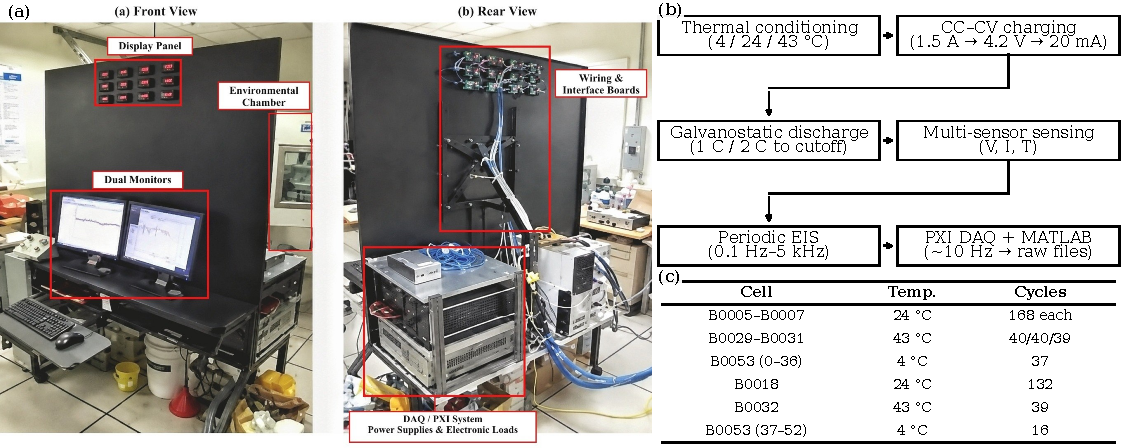
\includegraphics[width=\linewidth]{figs/fig2_nasa_experimental_setup.pdf}
\caption{NASA PCoE battery-data acquisition concept reconstructed from the official dataset description~\cite{saha2007battery}. This is an original schematic of the measurement chain, not a photograph of the physical apparatus.}
\label{fig:nasa_setup}
\end{figure}

\begin{table}[t]
\caption{NASA cycle counts used in the completed experiments.}\label{tab:nasa_stats}
\begin{tabular*}{\tblwidth}{@{}LLLL@{}}
\toprule
Cell & Ambient $T$ & Cycles used & Role \\
\midrule
B0005 / B0006 / B0007 & $24\,^\circ$C & $168$ each & Train \\
B0029 / B0030 & $43\,^\circ$C & $40$ each & Train \\
B0031 & $43\,^\circ$C & $39$ & Train \\
B0053 (0--36) & $4\,^\circ$C & $37$ & Train \\
B0018 & $24\,^\circ$C & $132$ & Unseen-cell test \\
B0032 & $43\,^\circ$C & $39$ & Unseen-cell test \\
B0053 (37--52) & $4\,^\circ$C & $16$ & Temporal test \\
\bottomrule
\end{tabular*}
\end{table}

\subsubsection{Evaluation Task Setup}
\label{sec:nasa_task_setup}

The NASA case study answers two complementary questions under one split. Unseen-cell generalization asks whether a model trained on B0005--B0007, B0029--B0031, and early B0053 can estimate SOH on B0018 and B0032. Temporal extrapolation asks whether the same model can continue the late-life segment of B0053 after seeing only cycles 0--36. The two settings are not equivalent: B0053 is partially observed, and the late tail contains only 16 cycles.

\subsubsection{Results and Analysis}
\label{sec:nasa_results}

E01 supplies the proposed-model reference (macro RMSE $0.0168$, MAE $0.0141$, $R^2$ $0.870$) that is reused as the frozen E05 TE-Q-Transformer entry. E02--E04 isolate temperature encoding and the matched quantum representation and are discussed in Section~\ref{sec:further_study}. E05 is the scored contemporary comparison on the same NASA split (Figure~\ref{fig:main_performance}; Table~\ref{tab:main_benchmark}).

Under the E05 protocol, TE-Q-Transformer recorded the lowest macro-averaged RMSE ($0.0168$), MAE ($0.0141$), and MAPE ($1.56\%$), and the highest macro-averaged $R^2$ ($0.870$), among the evaluated models. The closest scored baseline on RMSE was QNN-GRU ($0.0304$). The ranking is not uniform at the cell level. CNN1D recorded a lower RMSE on unseen B0018 ($0.0255$ versus $0.0271$), whereas TE-Q-Transformer recorded the lowest RMSE on unseen B0032 ($0.0119$) and on the B0053 temporal holdout ($0.0113$). iTransformer had the highest baseline $R^2$ ($0.533$). QLSTM did not improve on LSTM ($0.0445$ versus $0.0416$). These comparisons use a single seed and a NASA-only split; they are not a statistical test and not an unseen-temperature study.

E06 retrains five designated models and evaluates trajectory behaviour (Figure~\ref{fig:nasa_generalization}; Table~\ref{tab:e06_cells}). The E06 TE-Q-Transformer macro RMSE is $0.02387$, which differs from the frozen E05 reference ($0.01678$). The two numbers come from different trainings (E05 frozen E01/E04 checkpoint with weight decay $0.05$; E06 independent run with weight decay $0.01$) and are not substituted for one another. In the E06 five-model comparison, TE-Q-Transformer had the lowest RMSE on B0018 ($0.02758$), B0032 ($0.02036$), and B0053-test ($0.02366$). On B0032, PatchTST and iTransformer had lower MAE ($0.01714$ and $0.01850$ versus $0.01886$). The B0053-test $R^2$ of $0.184$ is limited by the short 16-cycle tail; RMSE and MAE are the more informative measures on that segment.

E07 then repeats those five models across five seeds (Section~\ref{sec:multiseed_analysis}). The NASA case study therefore supports a protocol-specific aggregate advantage for the frozen reference model in E05, a retained but numerically different E06 retraining result, and non-negligible seed variability in E07.

\begin{figure*}[t]
\centering
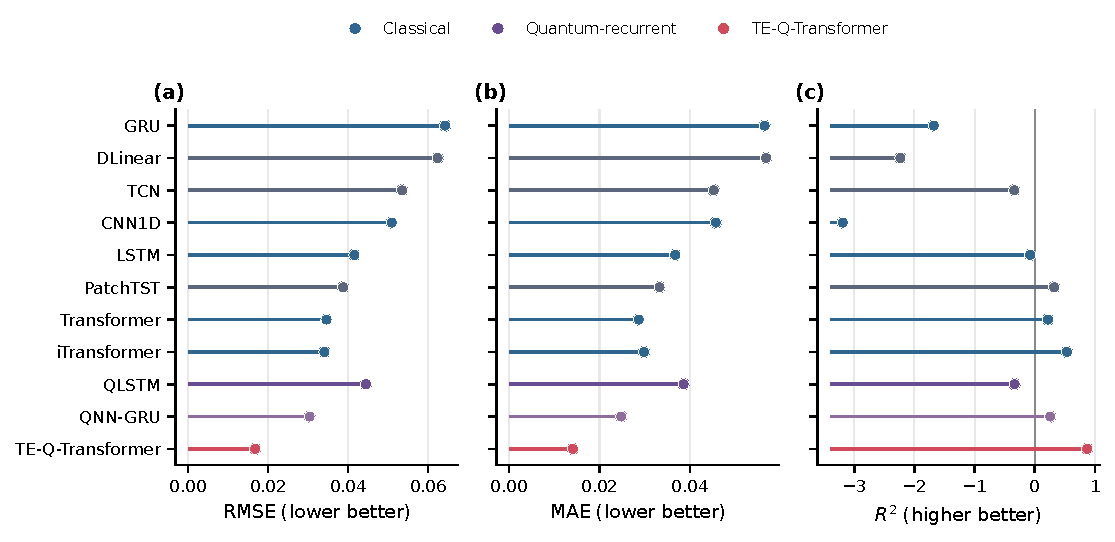
\includegraphics[width=\textwidth]{figs/fig6_main_performance.pdf}
\caption{E05 NASA macro-averaged performance for the ten scored baselines and the frozen TE-Q-Transformer reference. (a)~RMSE, (b)~MAE, (c)~$R^2$. Classical models are shown in blue/slate, quantum-recurrent baselines in purple, and TE-Q-Transformer in red. Single seed 42.}
\label{fig:main_performance}
\end{figure*}

\begin{figure*}[t]
\centering
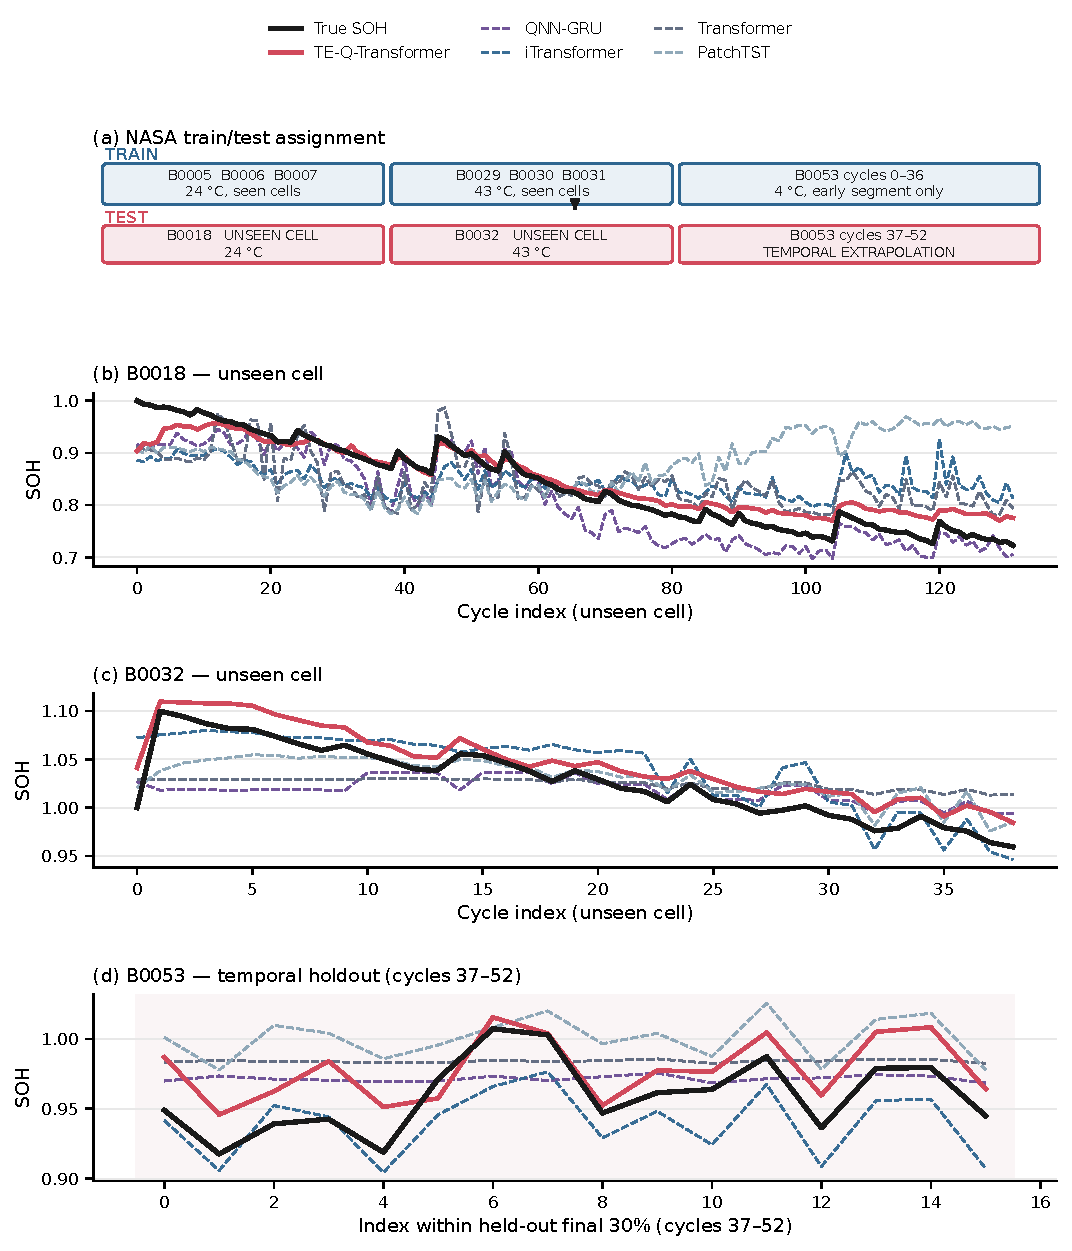
\includegraphics[width=\textwidth]{figs/fig9_nasa_generalization.pdf}
\caption{E06 predicted versus true SOH for the five designated models. (a)~B0018, unseen cell; (b)~B0032, unseen cell; (c)~B0053 cycles 37--52, temporal extrapolation. TE-Q-Transformer was retrained in E06 and is not the frozen E05 reference.}
\label{fig:nasa_generalization}
\end{figure*}

\subsection{External Validation on the CALCE Battery Dataset}
\label{sec:calce}

\subsubsection{Dataset Description}
\label{sec:calce_description}

CALCE CS2 cells from the University of Maryland~\citep{w9rg-7173-25} provide a second laboratory, chemistry, and cycling protocol. The CS2 series are prismatic lithium cobalt oxide cells (nominal $1.1$\,Ah) cycled with CCCV charge and $1$C discharge. Official Excel logs have no thermocouple column; temperature is filled at a constant $23\,^\circ$C ambient. The completed audit uses CS2\_35 ($n=880$), CS2\_36 ($n=968$), CS2\_37 ($n=1036$), and CS2\_38 ($n=1025$). Because ambient temperature is fixed, CALCE cannot support an unseen-temperature claim.

\subsubsection{Evaluation Protocol}
\label{sec:calce_protocol}

The audited CALCE experiment is zero-shot transfer of the frozen NASA TE-Q-Transformer checkpoint and the frozen NASA train-only scaler. All four CS2 cells are unseen external test cells. No CALCE-trained checkpoint, no CALCE scaler, and no CALCE hyperparameter search are used. This protocol is stricter than, and is not the same as, a CALCE-trained cross-cell split.

\subsubsection{Results and Analysis}
\label{sec:calce_results}

Table~\ref{tab:calce} and Figure~\ref{fig:calce_validation} report a negative transfer result. Pooled RMSE is $0.3325$, MAE $0.2676$, and $R^2$ $-1.789$ on $3909$ windows. Unweighted means over the four cells are RMSE $0.3302\pm0.0370$ and $R^2$ $-1.882\pm0.258$. Predictions remain near $1.01$ (documented range approximately $0.978$--$1.041$) while true SOH declines to about $0.14$. A constant predictor of $1.0$ has pooled RMSE $0.3277$, slightly lower than the frozen NASA model. Per-cycle prediction arrays were not archived; Figure~\ref{fig:calce_validation} therefore shows the audited true and predicted SOH ranges rather than reconstructed trajectories. The result is external cross-dataset evidence that the NASA-trained model does not track CALCE fade under zero-shot evaluation. It is not a CALCE-trained benchmark and not a temperature-generalization result.

\begin{table}[t]
\caption{NASA$\rightarrow$CALCE zero-shot results for the frozen TE-Q-Transformer. Lower RMSE/MAE and higher $R^2$ are better.}\label{tab:calce}
\begin{tabular*}{\tblwidth}{@{}LCCCC@{}}
\toprule
Cell & $n$ & RMSE~$\downarrow$ & MAE~$\downarrow$ & $R^2$~$\uparrow$ \\
\midrule
CS2\_35 & 880 & 0.2933 & 0.2415 & $-$2.070 \\
CS2\_36 & 968 & 0.3731 & 0.2937 & $-$1.567 \\
CS2\_37 & 1036 & 0.3483 & 0.2803 & $-$1.776 \\
CS2\_38 & 1025 & 0.3061 & 0.2524 & $-$2.115 \\
Pooled & 3909 & 0.3325 & 0.2676 & $-$1.789 \\
\bottomrule
\end{tabular*}
\end{table}

\begin{figure}[t]
\centering
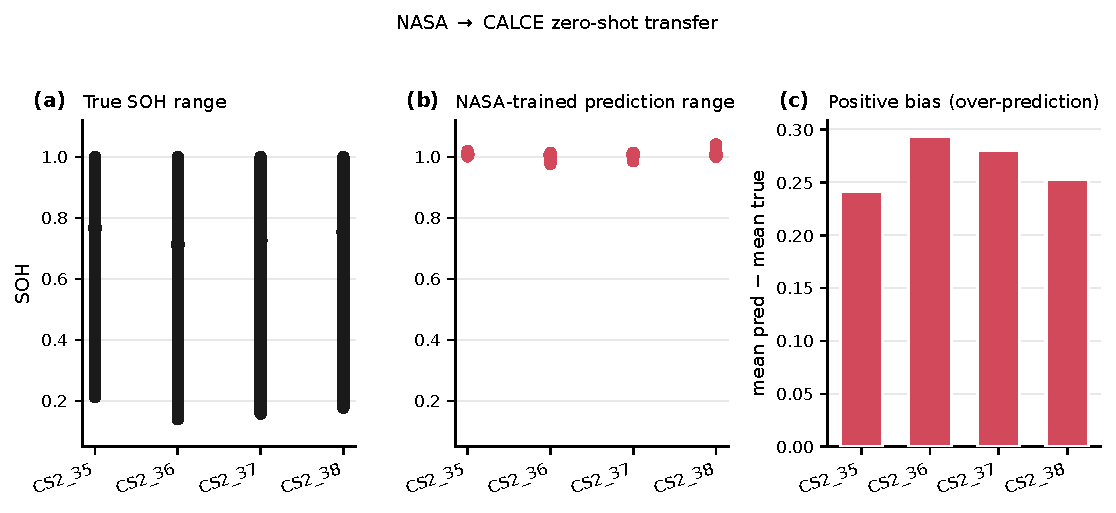
\includegraphics[width=\linewidth]{figs/fig12_calce_validation.pdf}
\caption{Audited NASA$\rightarrow$CALCE zero-shot ranges for (a)~CS2\_38 and (b)~CS2\_37. Black bars show the true SOH span; red bars show the frozen NASA prediction span. Per-cycle arrays were not archived.}
\label{fig:calce_validation}
\end{figure}

\subsection{Comparison with Contemporary Methods}
\label{sec:contemporary_comparison}

\subsubsection{Overall Benchmark Comparison}
\label{sec:overall_benchmark}

Table~\ref{tab:main_benchmark} lists the scored E05 metrics. TE-Q-Transformer achieved the lowest macro RMSE, MAE, and MAPE, and the highest macro $R^2$, among the evaluated models under the fixed NASA protocol. QNN-GRU is the nearest baseline on RMSE and MAE. Modern attention models (Transformer, PatchTST, iTransformer) occupy the next RMSE tier ($0.034$--$0.039$) with mixed $R^2$. Linear and convolutional baselines are weaker on the aggregate, and CNN1D and DLinear collapse on at least one evaluation setting (CNN1D $R^2=-10.45$ on B0053-test; DLinear $R^2=-7.16$ on B0032). The two quantum-recurrent models diverge: QNN-GRU is the strongest trained baseline, whereas QLSTM does not beat LSTM. E05 therefore does not support a generic quantum-module advantage. The contribution of the quantum embedding under matched physics is tested in E04, not in E05.

TE-Q MaxE in Table~\ref{tab:main_benchmark} is the true maximum absolute error on the $187$ test cycles ($0.1022$ on B0018). The stored reference CSV reports $0.0493$, which is the mean of the three cell-wise MaxE values and is not used here.

\begin{table*}[t]
\centering
\caption{E05 NASA main performance comparison. Overall metrics are unweighted means of B0018, B0032, and B0053-test. TE-Q-Transformer is the frozen E01/E04 reference (not retrained in E05). MaxE is the true maximum absolute error. TimesNet and QGRU are not scored.}\label{tab:main_benchmark}
\footnotesize
\begin{tabular}{@{}lccccccc@{}}
\toprule
Model & RMSE~$\downarrow$ & MAE~$\downarrow$ & MAPE~$\downarrow$ & $R^2$~$\uparrow$ & MaxE~$\downarrow$ & Params & Train (s) \\
\midrule
LSTM & 0.0416 & 0.0367 & 4.07 & $-$0.076 & 0.0904 & 71\,105 & 24.5 \\
GRU & 0.0642 & 0.0565 & 6.22 & $-$1.680 & 0.1631 & 54\,465 & 22.3 \\
CNN1D & 0.0509 & 0.0457 & 4.78 & $-$3.191 & 0.1245 & 47\,041 & 25.1 \\
TCN & 0.0535 & 0.0452 & 5.09 & $-$0.341 & 0.1491 & 91\,841 & 34.0 \\
DLinear & 0.0624 & 0.0568 & 5.88 & $-$2.232 & 0.1853 & 1\,031 & 15.5 \\
Transformer & 0.0346 & 0.0287 & 3.14 & 0.218 & 0.1123 & 80\,257 & 61.6 \\
PatchTST & 0.0387 & 0.0333 & 3.69 & 0.321 & 0.1457 & 109\,962 & 63.1 \\
iTransformer & 0.0341 & 0.0298 & 3.28 & 0.533 & 0.1165 & 137\,473 & 58.7 \\
QLSTM & 0.0445 & 0.0386 & 4.35 & $-$0.336 & 0.1066 & 37\,853 & 282.3 \\
QNN-GRU & 0.0304 & 0.0248 & 2.61 & 0.258 & 0.0725 & 29\,533 & 284.8 \\
TE-Q-Transformer$^{\mathrm{a}}$ & \textbf{0.0168} & \textbf{0.0141} & \textbf{1.56} & \textbf{0.870} & 0.1022 & 92\,554 & --- \\
\bottomrule
\end{tabular}
\vspace{2pt}
\begin{minipage}{\textwidth}
\footnotesize $^{\mathrm{a}}$Frozen reference. E05 training time $18.5$\,s is not comparable to the ten trained baselines and is omitted. True MaxE $=0.1022$ (B0018).
\end{minipage}
\end{table*}

\subsubsection{Computational Analysis}
\label{sec:computational_analysis}

Table~\ref{tab:compute} reports parameter counts and recorded wall-clock times. TE-Q-Transformer has $92\,554$ trainable parameters, comparable to TCN ($91\,841$) and Transformer ($80\,257$), and larger than QNN-GRU ($29\,533$). It is not described as lightweight. E05 classical training times are $15$--$63$\,s; QLSTM and QNN-GRU require about $283$--$285$\,s on the simulator. Independent from-scratch TE-Q training in E06 required $564.7$\,s on CUDA. E04, which matches classical and quantum embeddings on CPU \mbox{\texttt{default.qubit}}, required $2179.9$\,s (classical + physics) versus $3599.3$\,s (quantum + physics). These times are simulated execution cost, not physical quantum-hardware cost, and do not support a computational quantum-advantage claim. The observed trade-off is higher simulation time for a lower NASA macro error in E04 and E05.

\begin{table}[t]
\caption{Computational record. E05 times are the ten trained baselines. E06 TE-Q time is an independent CUDA retraining. Quantum rows use a classical simulator.}\label{tab:compute}
\begin{tabular*}{\tblwidth}{@{}LCCC@{}}
\toprule
Model & Params & Train (s) & Infer. (s) \\
\midrule
DLinear & 1\,031 & 15.5 & 0.022 \\
QNN-GRU$^{\mathrm{s}}$ & 29\,533 & 284.8 & 0.342 \\
QLSTM$^{\mathrm{s}}$ & 37\,853 & 282.3 & 0.341 \\
CNN1D & 47\,041 & 25.1 & 0.043 \\
GRU & 54\,465 & 22.3 & 0.029 \\
LSTM & 71\,105 & 24.5 & 0.038 \\
Transformer & 80\,257 & 61.6 & 0.070 \\
TCN & 91\,841 & 34.0 & 0.057 \\
TE-Q-Transformer$^{\mathrm{s}}$ & 92\,554 & 564.7$^{\mathrm{b}}$ & 0.766$^{\mathrm{b}}$ \\
PatchTST & 109\,962 & 63.1 & 0.052 \\
iTransformer & 137\,473 & 58.7 & 0.045 \\
\bottomrule
\end{tabular*}
\vspace{2pt}
{\footnotesize $^{\mathrm{s}}$PennyLane \mbox{\texttt{default.qubit}} simulation. $^{\mathrm{b}}$E06 CUDA retraining, not the E05 frozen reference.}
\end{table}

\subsection{Further Study}
\label{sec:further_study}

\subsubsection{Physics-Guided Temperature Analysis}
\label{sec:physics_analysis}
\label{sec:ablation}

E02 asks whether replacing raw/min--max temperature with the Arrhenius gate reduces NASA error (Figure~\ref{fig:physics_contribution}a; Table~\ref{tab:physics}). Physics-guided encoding lowers macro RMSE from $0.0201$ to $0.0168$ ($16.5\%$ relative). The cell pattern is mixed: RMSE increases on unseen B0018 ($-17.5\%$) and decreases on B0032 ($+34.8\%$) and B0053-test ($+40.4\%$). The B0018 deterioration is retained in the figure; the macro gain is not uniform.

E03 then isolates the two kinetic terms (Figure~\ref{fig:physics_contribution}b). Combined SEI + plating has the lowest E03 macro RMSE ($0.0215$), versus plating-only $0.0249$ and SEI-only $0.0330$. On B0053-test, plating-only is best (RMSE $0.0171$ versus combined $0.0222$). E02 physics-guided and E03 combined are separate trainings and are not averaged.

Learned activation-energy parameters from the E03 checkpoints are reported in Table~\ref{tab:ea} as optimized model scalars (initialized at $3.0$, i.e.\ $30$\,kJ\,mol$^{-1}$ in the implementation scale). They are not independently measured physical constants.

\begin{table}[t]
\caption{Physics-guided temperature ablation (macro of B0018, B0032, B0053-test). E02 and E03 are separate campaigns.}\label{tab:physics}
\begin{tabular*}{\tblwidth}{@{}LCCCC@{}}
\toprule
Variant & RMSE & MAE & MAPE & $R^2$ \\
\midrule
E02 raw $T$ & 0.0201 & 0.0171 & 1.84 & 0.723 \\
E02 physics-guided $T$ & 0.0168 & 0.0141 & 1.56 & 0.870 \\
E03 SEI-only & 0.0330 & 0.0282 & 2.88 & 0.068 \\
E03 plating-only & 0.0249 & 0.0208 & 2.21 & 0.592 \\
E03 SEI + plating & 0.0215 & 0.0172 & 1.81 & 0.610 \\
\bottomrule
\end{tabular*}
\end{table}

\begin{table}[t]
\caption{Learned activation-energy parameters from E03 (seed 42). Values are implementation-scale scalars, not measured $E_a$.}\label{tab:ea}
\begin{tabular*}{\tblwidth}{@{}LCCC@{}}
\toprule
Variant & Init. & $E_{a,\mathrm{sei}}$ & $E_{a,\mathrm{pl}}$ \\
\midrule
SEI-only & 3.0 & 2.618 & --- \\
Plating-only & 3.0 & --- & 2.180 \\
SEI + plating & 3.0 & 1.981 & 2.820 \\
\bottomrule
\end{tabular*}
\end{table}

\begin{figure*}[t]
\centering
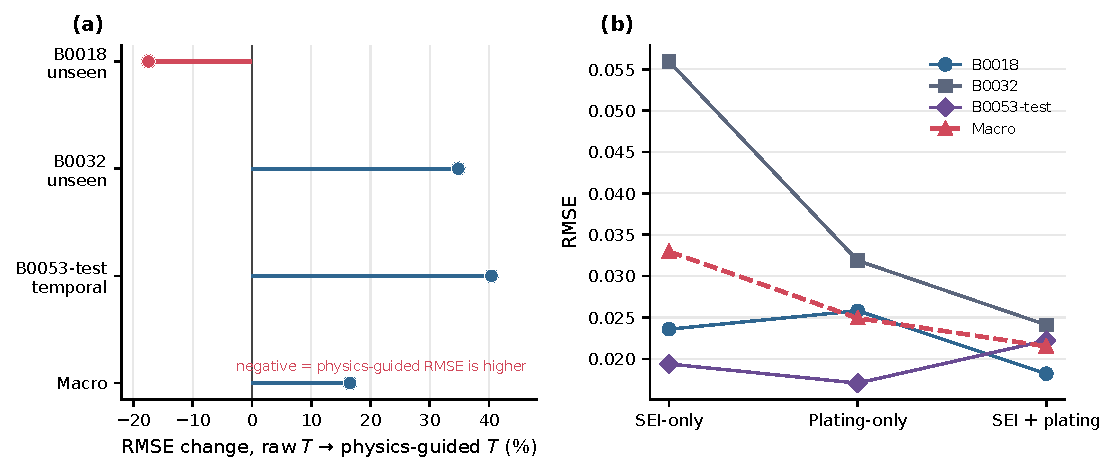
\includegraphics[width=\textwidth]{figs/fig7_physics_contribution.pdf}
\caption{Physics contribution. (a)~E02 percent RMSE change from raw temperature to physics-guided temperature; the B0018 bar is negative. (b)~E03 RMSE for SEI-only, plating-only, and combined pathways.}
\label{fig:physics_contribution}
\end{figure*}

\subsubsection{Quantum Representation Analysis}
\label{sec:quantum_analysis}

E04 holds the Arrhenius gate fixed and replaces the 4-qubit circuit with a capacity-matched classical MLP (Table~\ref{tab:e04}; Figure~\ref{fig:quantum_contribution}). Quantum + physics records macro RMSE $0.0215$ and $R^2$ $0.610$; classical + physics records $0.0431$ and $R^2$ $-0.746$. The quantum variant is better on all three NASA settings, including B0018. Parameter counts are nearly matched ($92\,554$ versus $92\,695$). Training on the CPU simulator is slower for the quantum model ($3599$\,s versus $2180$\,s). The result indicates additional predictive value of the simulated quantum representation under this matched protocol. It does not establish hardware speedup or a general quantum computational advantage.

\begin{table*}[t]
\centering
\caption{E04 matched classical versus quantum representation (macro metrics). MaxE is the maximum of the three cell-wise maxima. Training times are CPU PennyLane \mbox{\texttt{default.qubit}} simulation.}\label{tab:e04}
\footnotesize
\begin{tabular}{@{}lccccccc@{}}
\toprule
Variant & RMSE~$\downarrow$ & MAE~$\downarrow$ & MAPE~$\downarrow$ & $R^2$~$\uparrow$ & MaxE~$\downarrow$ & Params & Train (s) \\
\midrule
Classical + physics & 0.0431 & 0.0377 & 3.99 & $-$0.746 & 0.0912 & 92\,695 & 2179.9 \\
Quantum + physics & 0.0215 & 0.0172 & 1.81 & 0.610 & 0.0784 & 92\,554 & 3599.3 \\
\bottomrule
\end{tabular}
\end{table*}

\begin{figure}[t]
\centering
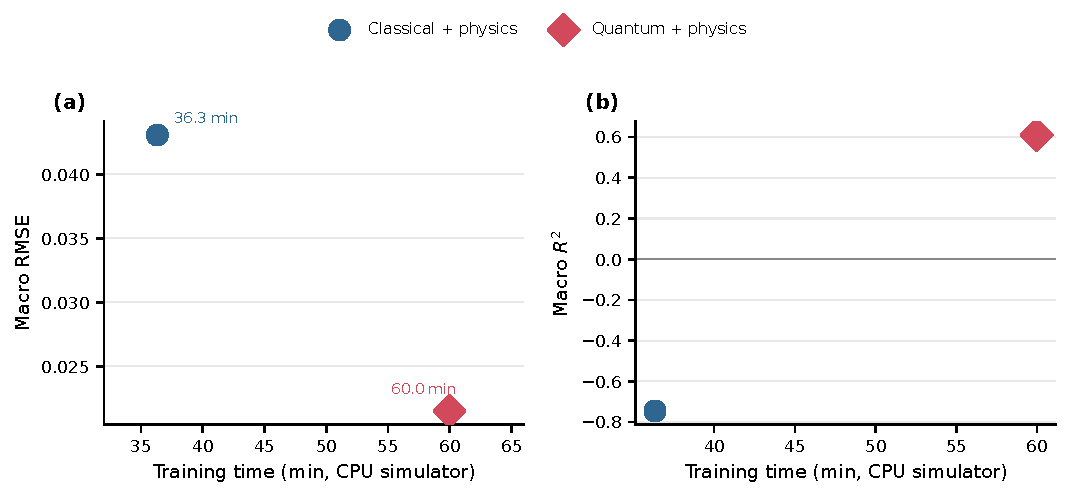
\includegraphics[width=\linewidth]{figs/fig8_quantum_contribution.pdf}
\caption{E04 accuracy--cost trade-off on the CPU PennyLane simulator. (a)~macro RMSE versus training time; (b)~macro $R^2$ versus training time.}
\label{fig:quantum_contribution}
\end{figure}

\subsubsection{Generalization Analysis}
\label{sec:generalization_analysis}

Table~\ref{tab:e06_cells} reports the E06 cell-wise scores. TE-Q-Transformer does not dominate every metric on every cell: PatchTST and iTransformer have lower MAE on unseen B0032, and several models remain close on the short B0053 tail. The unseen-cell mean RMSE for TE-Q-Transformer is $0.0240$ with a two-cell range of $0.0072$. QNN-GRU has a slightly smaller RMSE range ($0.0068$) at a higher mean ($0.0369$). These two-cell summaries describe observed variability only.

\begin{table*}[t]
\centering
\caption{E06 NASA cell-wise generalization for the five designated models. B0018/B0032 are unseen cells; B0053-test is temporal extrapolation.}\label{tab:e06_cells}
\footnotesize
\begin{tabular}{@{}lccccccccc@{}}
\toprule
 & \multicolumn{3}{c}{B0018 (unseen)} & \multicolumn{3}{c}{B0032 (unseen)} & \multicolumn{3}{c}{B0053-test (temporal)} \\
\cmidrule(lr){2-4}\cmidrule(lr){5-7}\cmidrule(lr){8-10}
Model & RMSE & MAE & $R^2$ & RMSE & MAE & $R^2$ & RMSE & MAE & $R^2$ \\
\midrule
TE-Q-Transformer & 0.0276 & 0.0215 & 0.890 & 0.0204 & 0.0189 & 0.713 & 0.0237 & 0.0209 & 0.184 \\
QNN-GRU & 0.0404 & 0.0344 & 0.765 & 0.0335 & 0.0248 & 0.221 & 0.0286 & 0.0241 & $-$0.195 \\
iTransformer & 0.0691 & 0.0624 & 0.311 & 0.0236 & 0.0185 & 0.613 & 0.0241 & 0.0214 & 0.154 \\
Transformer & 0.0604 & 0.0539 & 0.472 & 0.0335 & 0.0283 & 0.223 & 0.0358 & 0.0303 & $-$0.870 \\
PatchTST & 0.1249 & 0.1061 & $-$1.253 & 0.0222 & 0.0171 & 0.660 & 0.0449 & 0.0410 & $-$1.937 \\
\bottomrule
\end{tabular}
\end{table*}

\subsubsection{Multi-Seed Robustness}
\label{sec:multiseed_analysis}

E07 repeats the five E06 models on seeds 42--46 (Figure~\ref{fig:multiseed}; Table~\ref{tab:e07}). TE-Q-Transformer has the lowest mean RMSE ($0.0244\pm0.0096$) but a large coefficient of variation ($0.394$). Seed 43 is an adverse run (overall RMSE $0.0405$, B0032 $R^2=-2.13$). Seed 44 is the best TE-Q run (RMSE $0.0150$). QNN-GRU is more stable (RMSE $0.0381\pm0.0039$) at a higher mean error. Five predefined seeds do not constitute a statistical significance test, and the observed spread does not support a claim of uniform robustness.

\begin{table}[t]
\caption{E07 multi-seed robustness (mean $\pm$ SD over seeds 42--46). SD is the sample standard deviation, $n=5$.}\label{tab:e07}
\begin{tabular*}{\tblwidth}{@{}LCCC@{}}
\toprule
Model & RMSE & MAE & $R^2$ \\
\midrule
TE-Q-Transformer & $0.0244\pm0.0096$ & $0.0197\pm0.0084$ & $0.455\pm0.534$ \\
QNN-GRU & $0.0381\pm0.0039$ & $0.0328\pm0.0040$ & $-0.432\pm0.467$ \\
iTransformer & $0.0379\pm0.0112$ & $0.0327\pm0.0103$ & $0.133\pm0.733$ \\
Transformer & $0.0367\pm0.0071$ & $0.0312\pm0.0063$ & $0.167\pm0.298$ \\
PatchTST & $0.0466\pm0.0150$ & $0.0389\pm0.0126$ & $0.125\pm0.520$ \\
\bottomrule
\end{tabular*}
\end{table}

\begin{figure}[t]
\centering
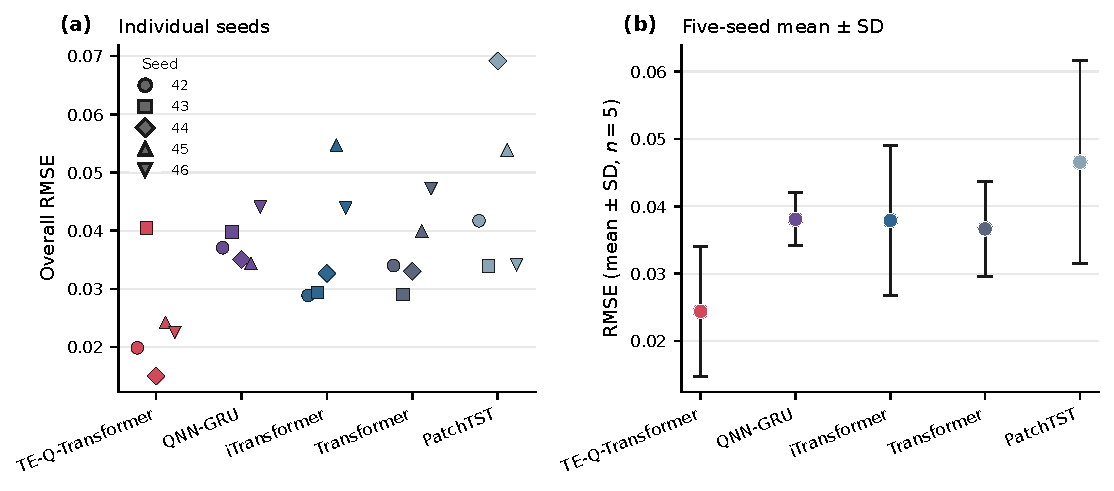
\includegraphics[width=\linewidth]{figs/fig11_multiseed_robustness.pdf}
\caption{E07 robustness. (a)~overall RMSE for each seed; (b)~mean $\pm$ SD over five seeds. TE-Q-Transformer seed 43 is the high-error red point.}
\label{fig:multiseed}
\end{figure}

\paragraph{Supplementary architectural ablation.}
Table~\ref{tab:s1_arch} retains the previously audited component ablation of the proposed architecture (rich entangler, temporal convolution, positional encoding, and CLS pooling). It is not an E02--E07 substitute and is not used to rank contemporary baselines.

\begin{table*}[t]
\centering
\small
\caption{Supplementary Table S1. Architectural component ablation on the NASA macro split (existing audited study). $\Delta$RMSE is relative to the full model.}\label{tab:s1_arch}\label{tab:nasa_ablation}
\begin{tabular}{@{}llcccccc@{}}
\toprule
Settings & Configuration & RMSE & MAE & MAPE & $R^2$ & MaxE & $\Delta$RMSE \\
\midrule
Basic entangler & Rich $\rightarrow$ basic & 0.0388 & 0.0320 & 3.53 & 0.342 & 0.0743 & $+0.0221$ \\
Pauli feature map & $+$ Pauli map & 0.0206 & 0.0166 & 1.78 & 0.774 & 0.0603 & $+0.0038$ \\
No temporal conv & $-$ temporal conv & 0.0261 & 0.0231 & 2.50 & 0.618 & 0.0554 & $+0.0093$ \\
GRU smoother & GRU replaces conv & 0.0274 & 0.0217 & 2.38 & 0.649 & 0.0610 & $+0.0107$ \\
No PE & $-$ positional encoding & 0.0330 & 0.0268 & 2.87 & 0.174 & 0.0862 & $+0.0162$ \\
Mean pooling & Mean pool, no CLS & 0.0237 & 0.0190 & 2.02 & 0.565 & 0.0642 & $+0.0069$ \\
Residual MLP & $+$ residual MLP & 0.0255 & 0.0214 & 2.29 & 0.545 & 0.0628 & $+0.0087$ \\
Full model & Rich, PE, conv $k{=}3$, CLS & 0.0168 & 0.0141 & 1.56 & 0.870 & 0.0493 & --- \\
\bottomrule
\end{tabular}
\end{table*}

\section{Threats to Validity}\label{sec:threats}

\subsection{External Validity}\label{sec:external}
The empirical findings are limited to the NASA PCoE and CALCE laboratory cells used in this study. The training and test cells within each dataset share a common experimental setting, and while CALCE gives a second chemistry and test bench, both datasets are still small-format laboratory cells cycled under controlled conditions.
% and do not cover pack-level behaviour, field duty cycles, or other open datasets. 
Ambient temperatures on the NASA held-out set span 4\,$^\circ$C, 24\,$^\circ$C, and 43\,$^\circ$C, which supports a multi-temperature check but is still a sparse sample of real operating conditions; the CALCE cells, by contrast, are cycled at a single fixed temperature, so the CALCE result checks cross-chemistry generalization rather than the temperature range itself. Performance may therefore change under different chemistries, sampling rates, or vehicle-level data. 
The quantum part of the proposed architecture is also simulated in PennyLane rather than executed on physical quantum hardware.
% so reported gains should be read as evidence for the hybrid classical-simulation pipeline, not as a claim about near-term quantum devices.
In addition, the component ablation in Section~\ref{sec:ablation} was carried out on NASA only; we have not verified that every part of the design contributes in the same way on CALCE, so the CALCE result in Section~\ref{sec:calce} should be read as evidence for the full model rather than for each of its components individually.

\subsection{Internal Validity}\label{sec:internal}
We use a single fixed hybrid multi-temperature cross-cell held-out split rather than $k$-fold or leave-one-battery-out rotation. That choice reduces optimistic leakage from mixing cycles of the same cell across train and test.
% , but it also means the metrics depend on this particular partition. 
In particular, B0018 and B0032 are fully held out, whereas B0053 contributes early cycles to training and only its late 30\% to testing, so cold-temperature behaviour is not completely unseen. The CALCE split follows the same rule: CS2\_38 is fully held out, while CS2\_37 contributes its first 70\% of cycles to training and only its late 30\% to testing.
% All models share the same 512-step windows, train-only min-max scaling for voltage, current, and time, and raw Celsius temperature for the Arrhenius gate. 
% This equalizes the protocol, yet hyperparameter choices, training schedules, and our re-implementations of GRU, LSTM, Transformer, QNN-GRU, and QLSTM may still differ from the original papers that motivated those baselines. Residual differences in optimization or capacity could therefore contribute to the observed gaps alongside the proposed architecture.

\subsection{Construct Validity}\label{sec:construct}
SOH is defined as current measured capacity divided by each cell's first-cycle capacity. This is a standard laboratory construct. However, it does not capture impedance growth, power fade, or pack-level state of health used in some BMS settings. 
% The Arrhenius gate encodes temperature through trainable SEI and lithium-plating activation energies that shape rotation angles; those parameters are learned from data and are not constrained to measured physical constants, so the gate is physics-informed rather than a calibrated ageing model. 
Input windows use voltage, current, temperature, and normalized time only. Complementary health indicators such as incremental capacity features or impedance spectra are outside the present construct. 

% Finally, RMSE, MAE, and R\textsuperscript{2} on window-level predictions summarize point error and fit on the combined test split; they do not alone certify cycle-life prognosis or safety-critical deployment readiness.

\section{Conclusion}
\label{sec:conclusion}
Reliable battery health monitoring is essential for ensuring the safety, performance, and longevity of lithium-ion battery-powered systems. Existing data-driven SOH estimation models do not adequately capture the effects of temperature on battery degradation, which limits their performance on unseen lithium-ion battery cells under different temperature conditions.
This work presents TE-Q-Transformer, a hybrid quantum-classical framework for lithium-ion battery SOH estimation that embeds Arrhenius-based thermal ageing into a four-qubit feature circuit before a compact transformer encoder. Here, temperature is mapped through trainable SEI and lithium-plating activation energies rather than treated as an ordinary scaled input, while voltage, current, and normalized time use $\pi$-scaled rotations. On the NASA dataset under a fixed hybrid multi-temperature cross-cell held-out protocol, TE-Q-Transformer achieved an RMSE of 0.0312, an MAE of 0.0257, and an R\textsuperscript{2} of 0.5164, outperforming five classical and hybrid quantum baselines and remaining the only model with a positive R\textsuperscript{2}. 
The results on held-out cells at 24\,$^\circ$C, 43\,$^\circ$C, and 4\,$^\circ$C further show closer tracking of gradual fade, steep mid-life drop, and short-cycle recovery. 
On the independent CALCE dataset, using the same cross-cell held-out protocol and the same six models, TE-Q-Transformer again gave the best result, with an RMSE of 0.0409, an MAE of 0.0334, and an R\textsuperscript{2} of 0.8704, ahead of GRU, LSTM, Transformer, QNN-GRU, and QLSTM.
These results indicate that physics-informed temperature encoding in the quantum stage can improve cross-cell SOH estimation under varying thermal conditions, and that the same architecture generalizes to a second dataset with a different chemistry and cycling protocol. 

Future work will extend the evaluation to more diverse laboratory and field datasets,including broader temperature ranges and different battery chemistries. Further improvements will explore hardware-efficient quantum circuits, noise-aware training, and more advanced physics-informed mechanisms to enhance scalability, robustness, and cross-battery generalization.

% To print the credit authorship contribution details

\printcredits

\section*{Declaration of generative AI tools use in the writing process}
During the preparation of this manuscript, the authors used ChatGPT to improve the language and readability of the text. The authors reviewed and verified all content and take full responsibility for the final manuscript.
%% Loading bibliography style file
\bibliographystyle{model1-num-names}

% Loading bibliography database
\bibliography{cas-refs}

% Biography
%\bio{}
% Here goes the biography details.
%\endbio

%\bio{pic1}
% Here goes the biography details.
%\endbio

\end{document}